\documentclass{beamer}
\usetheme{CambridgeUS}

%\usepackage{listings}
%\lstset{language=bash}

\usepackage[english,francais]{babel}
\usepackage[utf8]{inputenc}
%\usepackage[latin1]{inputenc}
\usepackage{verbatim}
%\usepackage{isolatin1}
%

% TODO
% * compris temps de réponse rendement
% * schema regle d'admission
% * photo icluster
% * MPI affinité processeurs
% * multicluster lien avec la hierarchy
% * Exemple de fichier de configuration OAR/MAUI
% * DRMAA / Globus / G-lite
% * notion d'éco-système / de co-système (vision intégré à cluster vision / Bull /serviware ) on 
% * on retombe dans les 80/20 (le tuning et la personnalisation reste et restera une affaire délicate)
% * Comparaison
% * Récursivité
% * Loadbalancing / timesharing / récusivité => Ordo
% * politique temporelle
% * Perspective / future
% * GUI
% * resoumission / dependance / job array / signaliation 
% * checkpointing / migration 
% * Comparaison
% * Lanceur parallèle 
% * filtrage / contraintes topologiques différences

\title{Propos sur les gestionnaires de tâches et de ressources ({\em Batch Scheduler})}
\author{Olivier~Richard (Mdc)}
\institute{ Laboratoire d'Informatique de Grenoble (LIG)\\
 Equipe-Projet INRIA Mescal}

\begin{document}

\frame{
	\titlepage
    \begin{center}
        %\vspace{2ex}
        
\includegraphics[height=6ex]{img/LIG_coul.jpg}
        \hspace{2ex}
        
\includegraphics[height=3ex]{img/cnrs.jpg}
        \hspace{1ex}
        
\includegraphics[height=3ex]{img/logo_inpg.jpg}
        \hspace{1ex}
        
\includegraphics[height=3ex]{img/inria.jpg}
        \hspace{1ex}
        
\includegraphics[height=3ex]{img/logo_ujf.jpg}
        \hspace{1ex}
        
\includegraphics[height=5ex]{img/logo_upmf.jpg}
    \end{center}
	}
\frame{
  \frametitle{Notre expérience}

  \begin{itemize}
    \item OAR: Gestionnaire de ressource
    \item Kadeploy: Outils de déploiment
    \item Cigri: Gestionnaire pour grille légère
  \end{itemize}

  \begin{itemize}
    \item CIMENT: Grappe de production
    \item Grid'5000: Plate-forme distribuée dédiée à l'expérimentation 
  \end{itemize}

  \begin{center}
    
\includegraphics[width=4cm]{img/Logo_Aladdin.png}
  \end{center}



}


\frame{
  \frametitle{Sommaire}
  	\tableofcontents
}

\section{Introduction}


\frame{
	\frametitle{Evolutions des grappes (clusters)}
	\begin{itemize}
		\item Démocratisation
		\item Densification	
		\begin{itemize}
			\item Nombre de processeurs en augmentation
			\item Nombre de coeurs (bi-processeurs / bi-coeurs) x4, x8 ... 
			\item \textbf{la puissance électrique}
		\end{itemize}
    \item Consommation électrique
	\end{itemize}
}

%\frame{
%  \frametitle{Utilisation}
%  \begin{itemize}
%    \item 1 utilisateurs: OK (gaspillage +++) 
%    \item 2 utilisateurs: on coupe la machine en 2 (gaspillage ++)
%    \item 3 à 5 utilisateurs: partage par mail (frustration , grosse colère, gaspillage +)
%    \item au-delà mise en place d'un gestionnaire de tâches et de ressources 
%  \end{itemize}
%  Partage et allocation des ressources suivant les requêtes des utilisateurs 

%%% TODO rajoute un dessin ici

%}


\frame{
 \frametitle{Les grappes au quotidien}


{\bf Des utilisateurs et des programmes:}
  \begin{itemize}
		\item Utilisateurs avec une connaissance très variable des aspects systèmes / gestion des ressources 
		\item Les tâches à exécuter sont variées (nombre, taille, durée...)
	\end{itemize}

{\bf Les ressources reste(ro)nt limitées}
{\bf Rôles de l'administrateur:}

 \begin{itemize}
	\item Aider les utilisateurs à exploiter les ressources de calcul (et de stockage)
	\item Maintenir un bon niveau d'utilisation de(s) grappe(s)
 \end{itemize}
}


\frame{
 \frametitle{Nécessité d'un gestionnaire de tâches et de ressources}

Organiser/répartir manuellement les ressources entre les utilisateurs et leurs tâches à traiter est réaliste qu'à {\bf petite échelle}, moins de 10 utilisateurs et peu de tâches en concurrence ({\em agenda partagé, mailing-list}).
\\[0.5cm]

A {\bf moyenne et grande échelle} on utilise un gestionnaire de ressource

\begin{itemize}
	\item gére l'attribution des ressources aux tâches suivant une politique préétablie
	\item fait le suivi de l'exécution des tâches
	\item surveille l'état des ressources
\end{itemize}
{\bf Attention: l'administrateur est toujours nécessaire !!}
}

\begin{frame}
	\frametitle{Principe général}

	Dans leur version simple, séparation en 2 couches (parfois une 3éme Workload Managment) :
	
	\begin{center}
			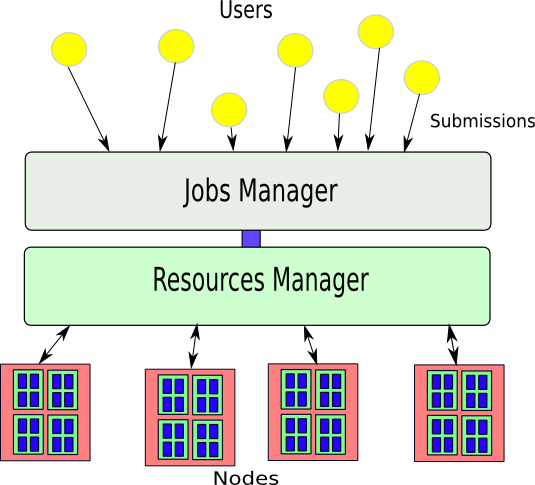
\includegraphics[width=7cm]{img/task_resources.png}
	\end{center}

\end{frame}





\frame{
  \frametitle{Mise en place}

\begin{block}{}
  \begin{itemize}
    \item Lors de l'installation de la machines par la société la fournissant.
    \item Les paramétrages initiaux peuvent convenir sur la durée de vie la machine
    \item Reparamétrages si:
    \begin{itemize} 
      \item La population d'utilisateur change 
      \item Les tâches à exécuter évoluent en nature
      \item Mise-à-jour / ajout de matériel (exemple nouvelle tranche)
    \end{itemize}
  \end{itemize}
 \end{block}

  \begin{alertblock}{Important}
    L'installation et le paramétrage d'un gestionnaire suppose des échanges avec les utilisateurs et les adminstrateurs (réunion, information, formation, support). Il peut y avoir des compromis à déterminer (rendement/niveau de service) 
  \end{alertblock}
}


\frame{
 \frametitle{Les Gestionnaires de tâches et de ressources}
	
	Aussi appelés {\em Batch Scheduler}
	
	Existent en très grand-nombre:

	  \begin{itemize}
    \item {\bf Condor } 
		\item {\bf Sun Grid Engine (SGE)} 
    \item {\bf MAUI/Torque} 
    \item {\bf Slurm} 
    \item {\bf OAR} (LIG/INRIA) :)

    \item LSF (Platform) 
    \item PBS Pro
    \item Moab (Cluster Resources)
    \item Autres: {\bf BQS (CC-IN2P3)}, {\bf Lava}, Loadleveler, CCS...
 \end{itemize}
  \begin{itemize}
    \item \url{http://en.wikipedia.org/wiki/Job_scheduler}
  \end{itemize}

	{\bf Note:} Ici calcul haute-performance/grappe, mais utilisés dans d'autre domaine gestion/finance/rendu de film (enchainement de tâches). 

}


\section{Principes}

\begin{frame}
	\frametitle{Principe général}

	Dans leur version simple, séparation en 2 couches (parfois une 3éme Workload Managment) :
	
	\begin{center}
			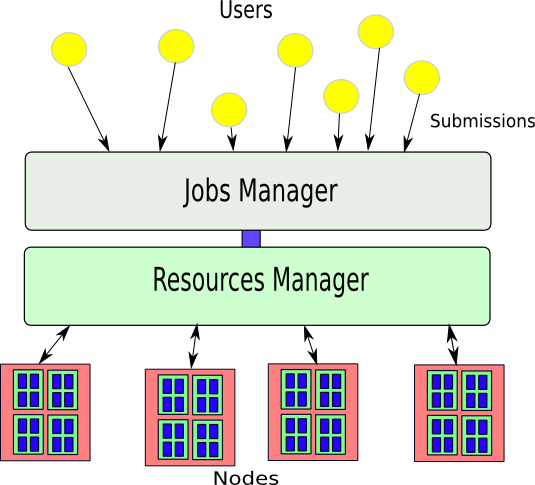
\includegraphics[width=7cm]{img/task_resources.png}
	\end{center}

\end{frame}

\begin{frame}
	\frametitle{Organisation générale}

	\begin{itemize}
		\item Un serveur central
		\item Des programmes clients (en ligne de commandes) pour l'interaction avec les utilisateurs
		\item Une grande latitude dans le paramétrage
	\end{itemize}

	\begin{center}
		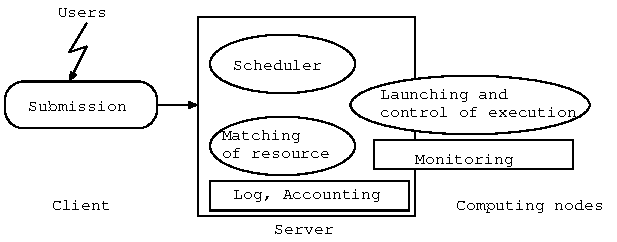
\includegraphics[height=4cm]{Batch_organization.pdf}
	\end{center}

\end{frame}


\section{Fonctionnaliés}

\begin{frame}
\frametitle{Fonctionnalités (1/2)}
	{\bf liste non-exhaustive}
		\begin{itemize}
		\item Tâche ({\em soumission}) Interactive (shell) / Batch
		\item Tâche séquentielle et parallèle
		\item Walltime (temps limite). ({\bf important pour l'ordonnancement)}
		\item Accès exéclusif / non-exclusif aux ressources 
		\item Appariement de ressources
		\item Scripts Epilogue/Prologue (exécuter avant/après les tâches)
		\item Suivi ({\em monitoring} des tâches (consommation des ressources)
		\item Dépendance entre tâches ({\em workflow})
		\item Logging et accounting
		\item Suspension/reprise des tâches 
	\end{itemize}
\end{frame}

\begin{frame}
\frametitle{Fonctionnalités (2/2)}
	{\bf liste non-exhaustive}
		\begin{itemize}
    \item Dépendance entre job
    \item Tableaux de tâches
    \item {\bf Advance Reservation }
		\item {\bf Expression des hiérarchies dans les requêtes }
		\item {\bf Support de ressources de type différent (ex licence, capacité de stockage, capacité réseaux...)  }
		\item {\bf Tâche container} ({\em soumettre dans une tâche})
		\item {\bf tâche besteffort}
		\item {\bf Type multiple de tâches} (besteffort, powersaving, deploy, timesharing, idempotent, {\bf power}, cosystem ...) (élément important pour l'extension/l'adaptation)
    \item Tâches moldables
		\item First-Fit (Conservative Backfilling,)
		\item Fairsharing 
		
	\end{itemize}
\end{frame}


\frame[plain]{
	\frametitle{OAR: un gestionnaire de taches et de ressources  {\bf polyvalent}}

  \vspace{-2.5cm}

  \begin{center}
    \hspace{9.5cm}
    \includegraphics[height=16ex]{img/oar_logo.png}
   \end{center} 

  \begin{center}
    \vspace{-0.5cm}
    {\bf http://oar.imag.fr/}
  \end{center}
}


\frame{
\frametitle{OAR: Historique}
%%% TODO rajoute image icluster
\begin{itemize}
  \item Début 2003: Une machine dans le Top500 (225 noeuds), OpenPBS(Torque) est instable et difficile à faire évoluer 
  \item PBSpro se comporte mieux (passage à l'échelle imparfait)
  \item Regle des 80/20 (20\% des fonctionnalités utilisées dans 80 \% des situations )
\end{itemize}

	\begin{center}
  	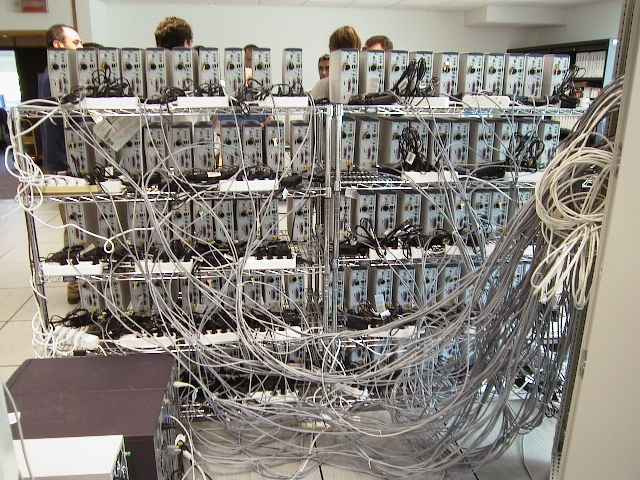
\includegraphics[width=6cm]{img/icluster1.jpg}
  \end{center}
}

\begin{frame}
	\frametitle{Objectifs}

	Un gestionnaire de tâches et de ressources {\bf polyvalent} et {\bf {\em personnalisable}}.

	\begin{itemize}
		\item Suivre l'évolution technologique (machine et infrastructure de plus en plus complexe)
		\item Adaptation aux différents contextes (cluster, cluster-on-demand, cluster virtuel, plate-forme pour l'expérimentation à la Grid'5000, {\em grand cluster}, besoin spécifique).
	\end{itemize}

\begin{alertblock}{Sous-estimation}
   Regle des 80/20 : les 20\% des fonctionnalités {\bf ne sont pas les mêmes pour tous !!!}  
\end{alertblock}

\end{frame}


%% Principe
\frame{
  \frametitle{OAR: principes de conception}
Utilisation de composants logiciels de haut niveau
   \begin{itemize}
    \item {\bf Base de donnée relationnelle} (MySql/PostgreSQL) pour stocker et échanger:
      \begin{itemize}
        \item Information sur les ressources et les tâches 
        \item L'état interne du système
       \end{itemize}
    \item {\bf Language(s) de script} (majoritairement Perl) pour le moteur d'exécution 
    \begin{itemize}
     \item Bien adapté pour les parties systèmes
     \item Structures de haut niveau (listes, tables associatives, tris...)
     \item Cycles de développement court
    \end{itemize}
    \item {\bf Autres composants} (Perl, Ruby, Caml) 
    \begin{itemize}
      \item \textbf{SSH, CPUSET} (confinement, nettoyage)
      \item \textbf{Taktuk} lanceur lui aussi très polyvalent
    \end{itemize}
  \end{itemize}

}

\frame{
	\frametitle{OAR : organisation générale}

	La base de donnée a un rôle central

	\begin{itemize}
		\item {\bf l'état interne simplement accessible}
		\item le moteur est composé de {\bf petit modules Perl}
		\item chaque module (= un script) peut-être facilement remplacé
	\end{itemize}

	\begin{center}
		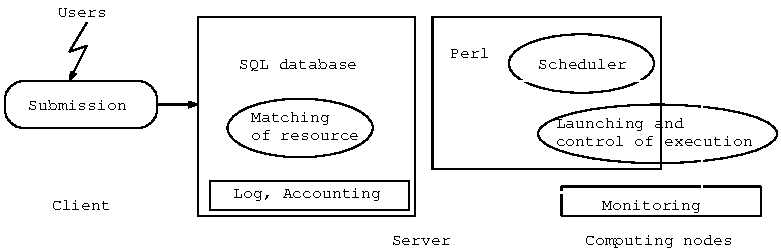
\includegraphics[height=3cm]{OAR_organization.pdf}
	\end{center}
}

\begin{frame}
\frametitle{Cycle de général}
	\begin{center}
		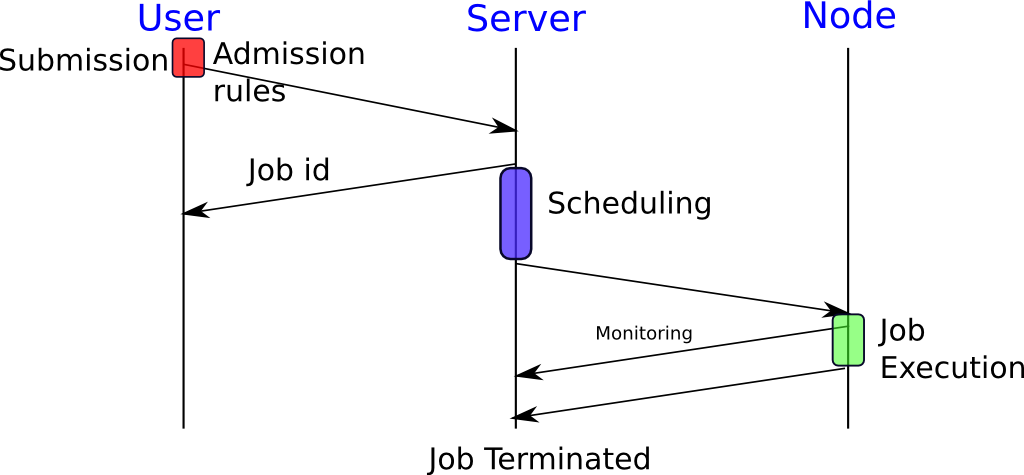
\includegraphics[width=10cm]{cycle_job.png}
	\end{center}
\end{frame}


\frame{
  \frametitle{Régles d'admissions}
  \begin{alertblock}{Un point de paramétrage important}
    \begin{itemize}
      \item {\bf Cadrage} des réquêtes
      \item fixe des valeurs par défaut: walltime, queue, nombre de ressources demandées, 
      \item contrôle d'accès (utilisateur, groupe, plage horaire...)
      \item point de {\em personnalisation} (au même titre que les scripts de prologue et d'épilogue)
    \end{itemize}
  \end{alertblock}
}


\frame{
	\frametitle{Diagramme d'état d'une tâche}
	Exemple du système OAR (version 1.6)
	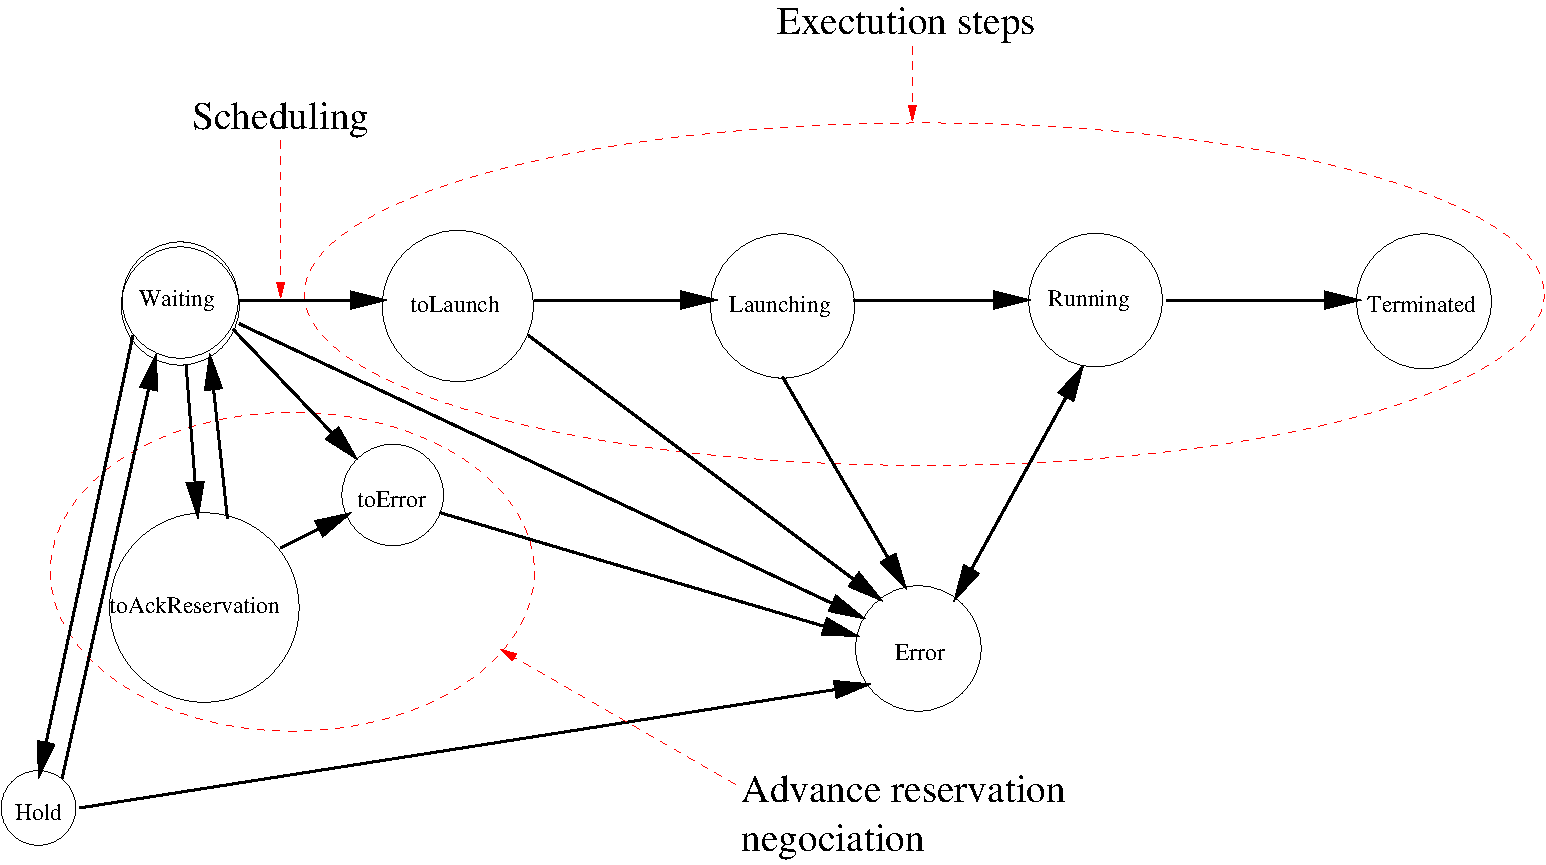
\includegraphics[width=\textwidth]{JobStates.pdf}
}

\begin{frame}
	\frametitle{Examples de soumission: OAR}
	
Soumission pour tâche interactive: \footnote{{\bf Note:} Chacune des commandes de soumission renseigne un numéro de tâche.}

		\begin{itemize}
			\item	{\bf oarsub -l nodes=4 -i}
		\end{itemize}

	Soumission en {\em batch} (avec {\em walltime} et choix de queue):
		\begin{itemize}
			\item	{\bf oarsub -q default -l walltime=2:00,nodes=10 /home/toto/script}
		\end{itemize}

	Soumission d'une réservation:
		\begin{itemize}
			\item	{\bf oarsub -r "2008-04-27 11:00" -l nodes=12}
		\end{itemize}

	Connection à une réservation (utilise le numéro de tâche):
		\begin{itemize}
			\item	{\bf oarsub -C 154}
		\end{itemize}


\end{frame}

\section{Ordonnancement}
% FIFO, BACKFILLING, FAIRSHARING, Advance reservartion, PRIORITE, BEST-EFFORT récursivité

\begin{frame}
	\frametitle{Ordonnancement}
	
	L'ordonnancement est l'étape \footnote{{\bf Note:} l'ordonnancement est recalculé à chaque changement d'état (majeur) d'une tâche.}
où le système choisi les {\bf ressources à attribuées} aux tâches et {\bf les dates de lancement}.
\\[0.4cm]
	L'ordonnancement est défini suivant une {\bf politique} qui se traduit par l'utilisation {\bf d'algorithmes d'ordonnancement}.
\\[0.4cm]
	{\bf De plus} de nombreux {\bf critères et paramètres} sont utilisés pour guider et cadrer les allocations et les priorités.
 

\end{frame}

\frame{
	\frametitle{Organisation de l'ordonnancement}
	Gestion des tâches par file (queues)
	\begin{itemize}
		\item chaque file a une priorité
		\item chaque file a sa propre politique d'ordonnancement
	\end{itemize}
%equivalent to scheduling jobs with priorities but easier to administrate
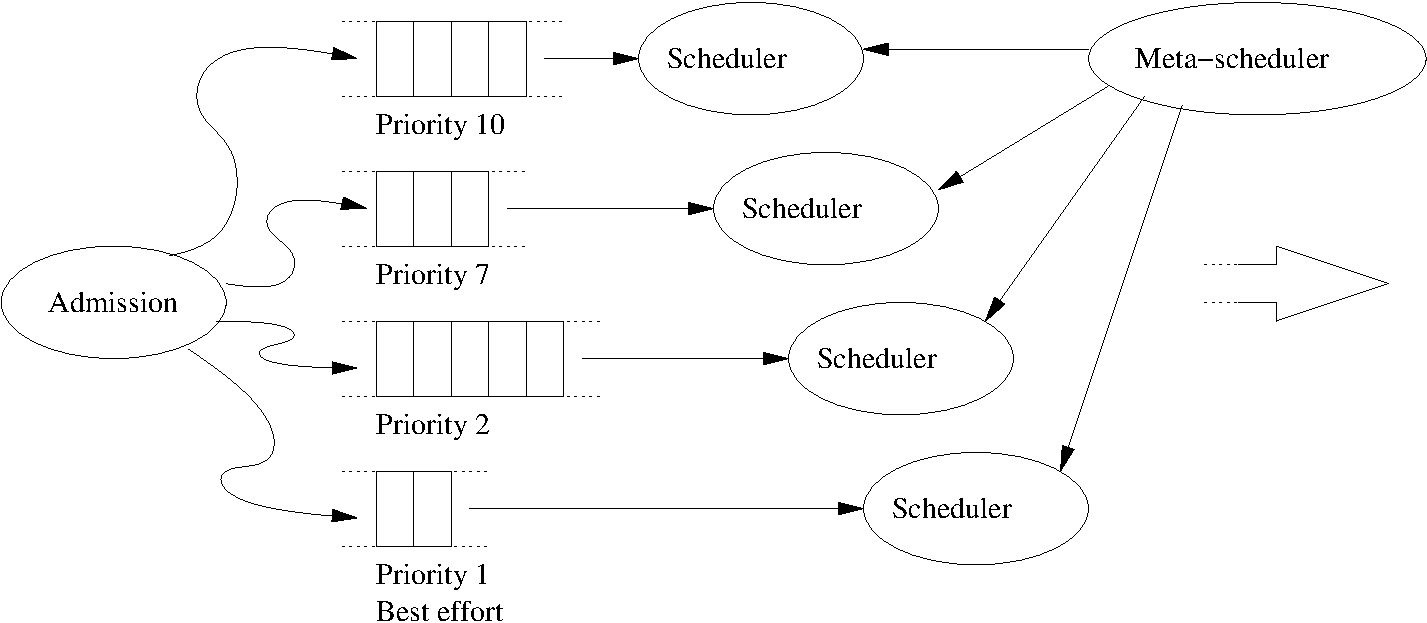
\includegraphics[width=\textwidth]{schedule_eng.pdf}
}

\frame{
	\frametitle{Appariement de ressource / ressource matching}

  \begin{block}{Une étape préliminaire à l'ordonnancement}
    \begin{itemize}
      \item {\bf Filtrage} de resources
      \item {\bf Classement} de ressource dans Condor 
      \item Permet de spécifier des besoins particuliers
      \item mémoire, architecture, machine particulières, OS, niveau de charge...    
    \end{itemize}
  \end{block}

  Condor / ClassAds : Syntaxe, Attributs, Opérateurs, Classement (Ranking)
}




\begin{frame}
	\frametitle{Politiques d'ordonnancement}
		\begin{itemize}
		\item FIFO (First-In First-Out)
		\item First-Fit (Backfilling)
		\item FairSharing
    \item Equilibrage de charge
    \item Récursivité
		\item SLA (Service Level Agrement)(Qualité de Sercice)
	\end{itemize}

\end{frame}

\begin{frame}
	\frametitle{FIFO: Fisrt-In First-Out}
	\begin{center}
		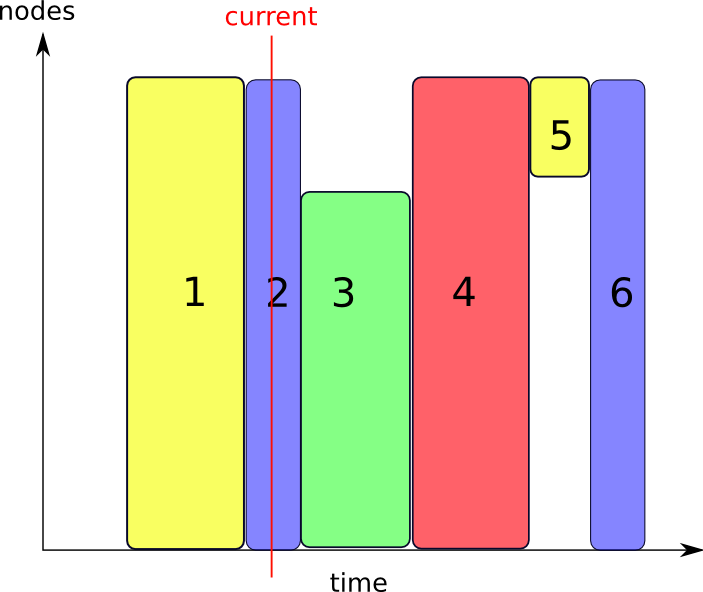
\includegraphics[width=7cm]{fifo.png}
	\end{center}

\end{frame}

\begin{frame}
	\frametitle{ First-Fit (Backfilling)}
	Remplissage des trous si l'ordre des tâches précédentes ne sont pas modifiées
	\begin{center}
			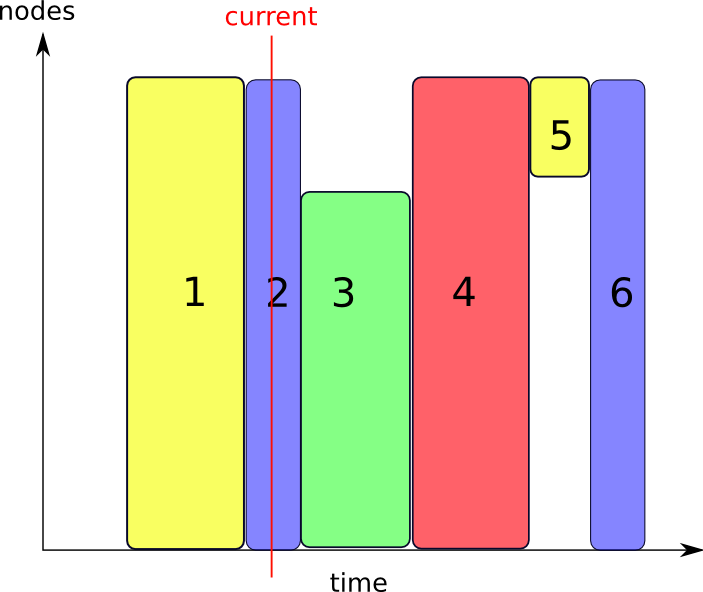
\includegraphics[width=6cm]{fifo.png}
		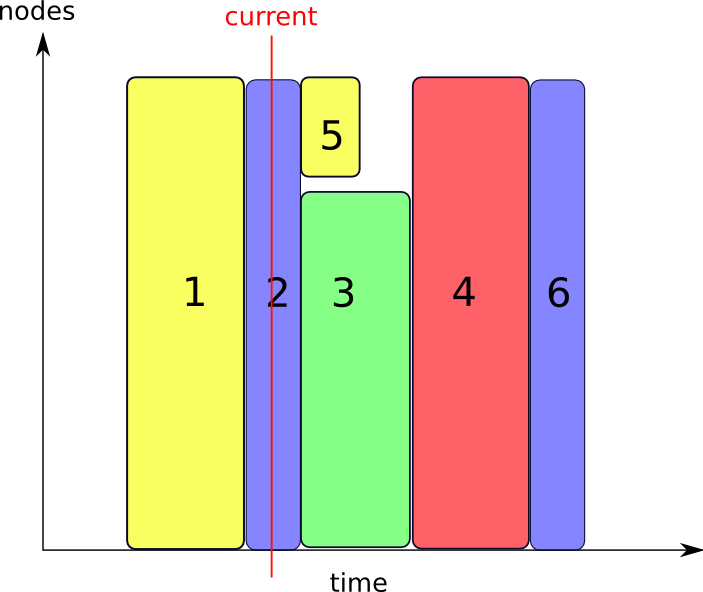
\includegraphics[width=6cm]{cbf.png}
	\end{center}

\end{frame}

\begin{frame}
	\frametitle{FairSharing (partage équitable)}
	L'ordre est calculé suivant ce qui a été consommé (on favorise les utilisateurs peu gourmands). Définition d'une fenêtre et paramètres de pondération.
	\begin{center}
		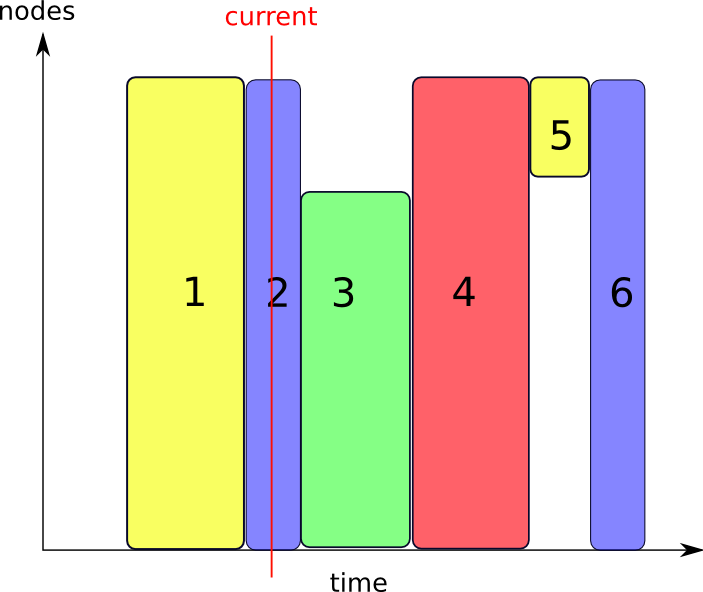
\includegraphics[width=6cm]{fifo.png}
		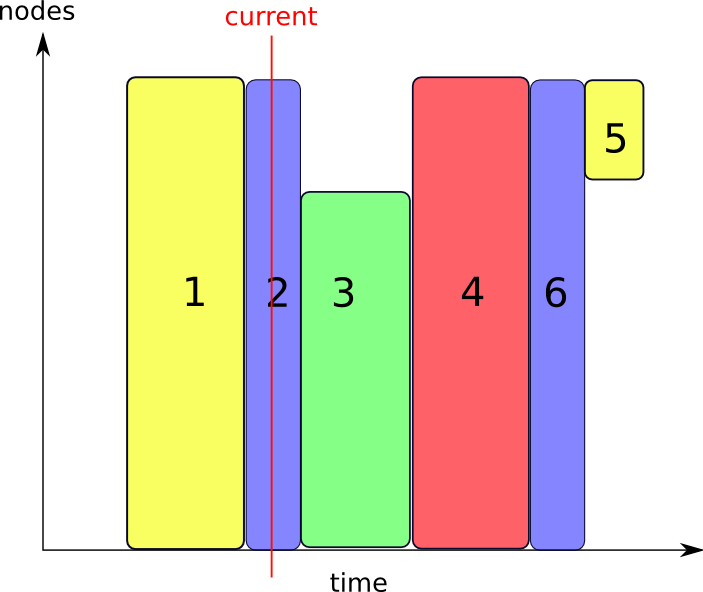
\includegraphics[width=6cm]{fairsharing.png}
	\end{center}
\end{frame}

\begin{frame}
	\frametitle{Réservation ({\em Advance Reservation})}

		\begin{itemize}
		\item {\bf Très pratique} pour démo, planification, tâche de type grille...
		\item {\bf Mais}
			\begin{itemize}
				\item Contraignant pour l'ordonnancement (attention au niveau d'utilisation)
				\item Les ressources sont rarement utilisée sur toute la durée (gaspillage)
			\end{itemize}
		\end{itemize}

	\begin{center}
		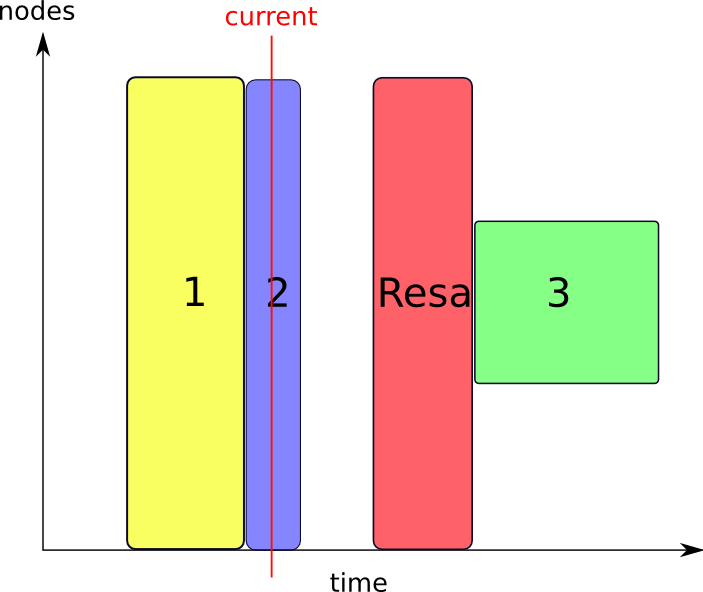
\includegraphics[width=6cm]{resa.png}
	\end{center}
	{\bf oarsub -r "2008-04-27 11:00" -l nodes=12}

\end{frame}

\begin{frame}
  \frametitle{Equilibrage de Charge}

  Une solution relativement simple :maintenir des indicateurs de charge et faire un tri en ordre croissant avant affectation. Attention peut interférer ou ne pas être possibles avec certains ordonnanceurs 
\end{frame}

\begin{frame}
  \frametitle{TimeSharing}
  
  \begin{center}
			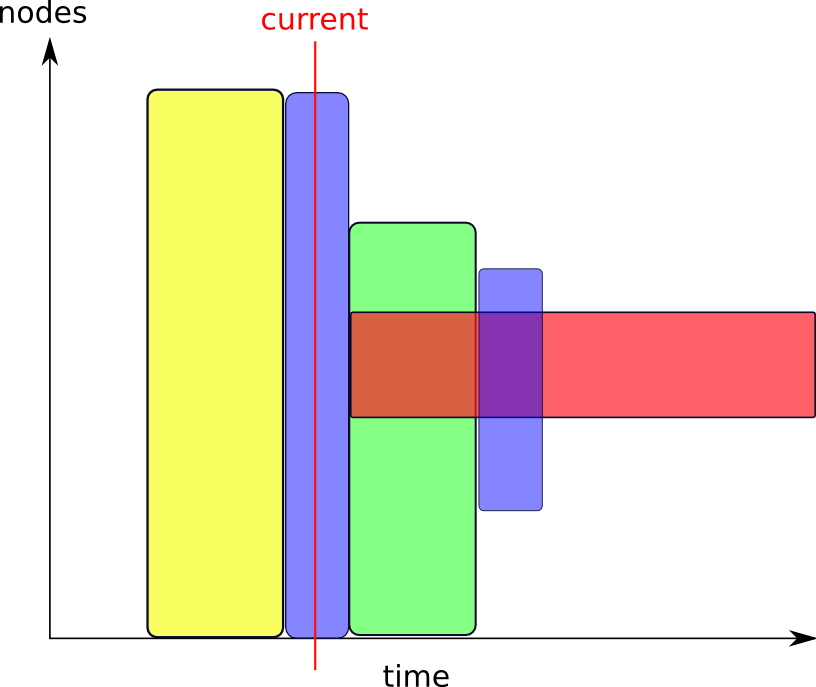
\includegraphics[width=7cm]{timesharing.png}
	\end{center}


\end{frame}

\begin{frame}
  \frametitle{Récursivité}
  Faire de l'ordonnancement dans une allocation/réservation. Intéressant pour formation, démo, partage de ressource plus flexible  par groupe d'utilisateurs / projet. Tâche de type container. 
  \begin{center}
			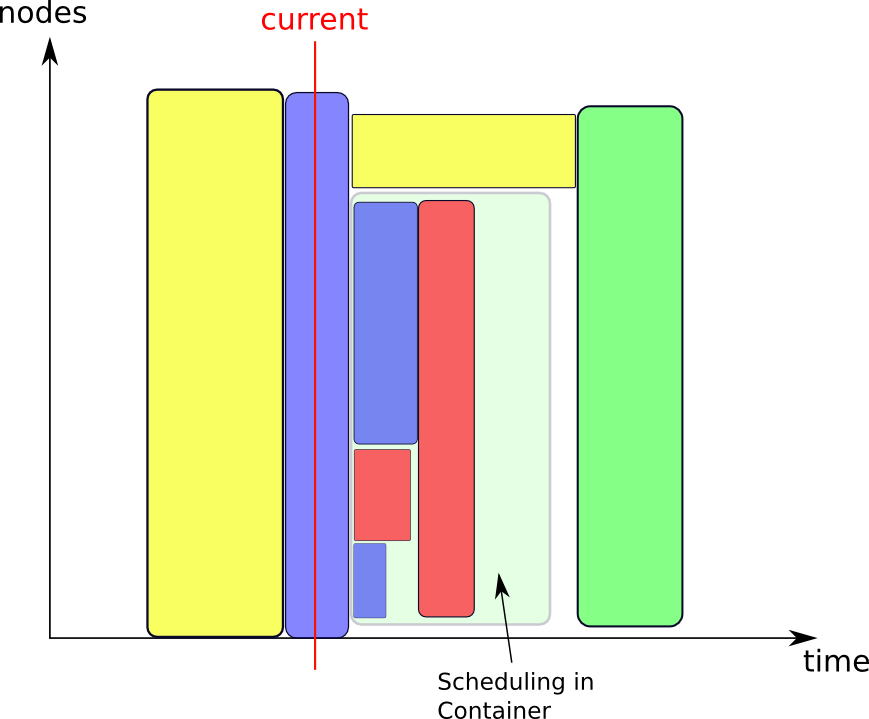
\includegraphics[width=7cm]{recursivity.png}
	\end{center}

\end{frame}






\section{Contraintes Topologiques}

\frame{
\frametitle{Contraintes Topologiques}
  \begin{block}{Evolution du matériel}
    \begin{itemize}
      \item switch/noeud/cpu/core: \alert{Architecture Hierarchique}
      \item machine NUMA / machine BlueGene grille 2D, 3D 
    \end{itemize}
  \end{block}
  \begin{center}
  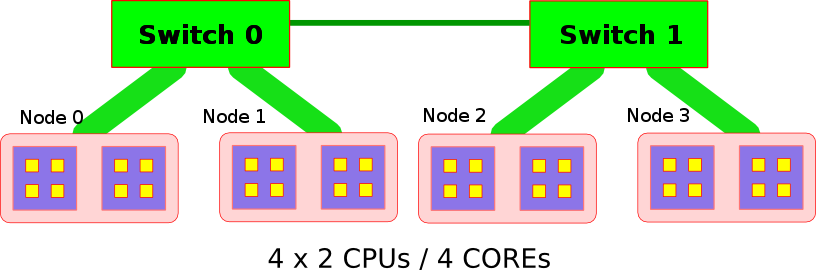
\includegraphics[width=9cm]{img/cluster_hierar.png}
  \end{center}
}

\frame{
\frametitle{Contraintes Topologiques: hiérarchique}
Problème avec les applications parallèles sensible au débit communication.
\begin{center}
  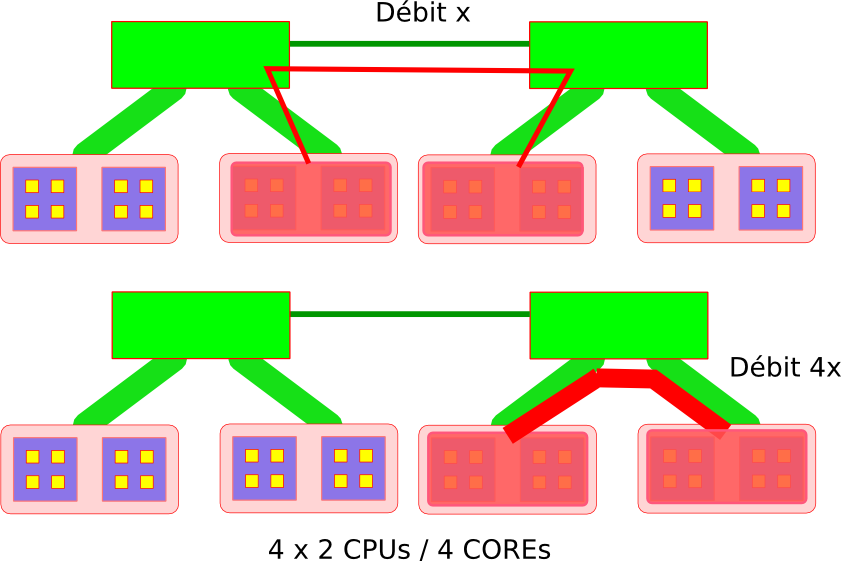
\includegraphics[width=9cm]{img/cluster_hierar_app.png}
  \end{center}
}

\frame{
\frametitle{Contraintes Topologiques: grille/tore 2D}
\begin{center}
  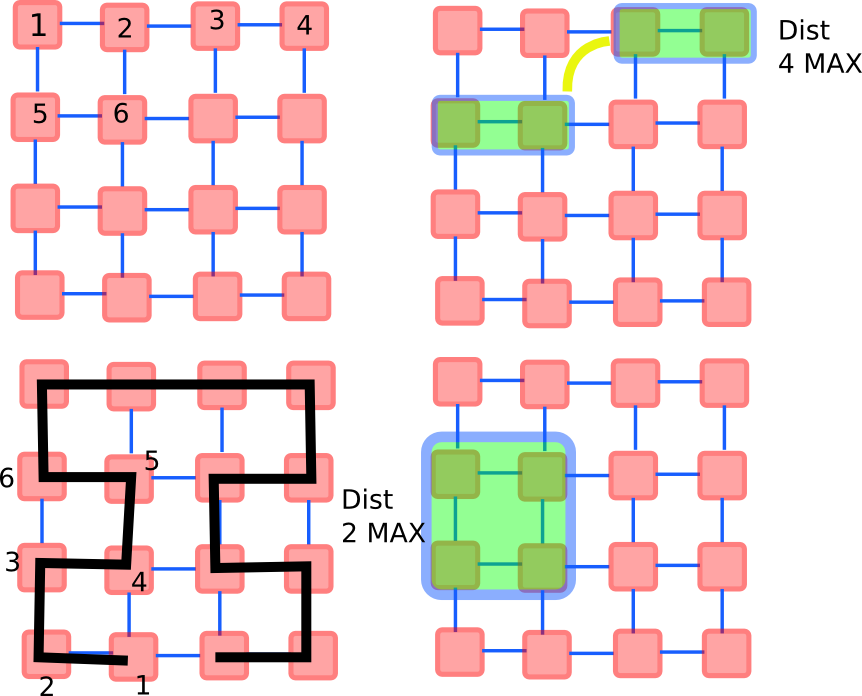
\includegraphics[width=9cm]{img/grille_2D_renum.png}
\end{center}
}

\frame{
\frametitle{Contraintes Topologiques: grille/tore 3D}
\begin{itemize}
  \item Courbe de Hilbert (Slurm / topology)
  \item Wikipedia / $Hilbert\_curve$ 
\end{itemize}
\begin{center}
  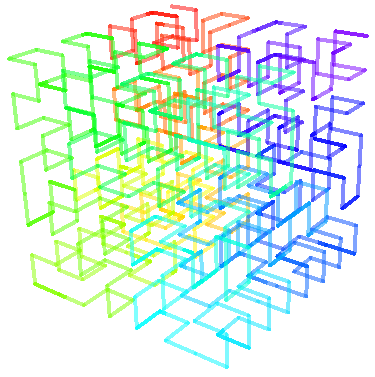
\includegraphics[width=7cm]{img/Hilbert3d-step3.png}
\end{center}
}

\frame{
\frametitle{Contraintes Topologies:}

\begin{block}{En résumé}
\begin{itemize}
  \item Les contraintes topologiques complexifient l'ordonnancement, problème d'optimisation
  \item L'ordonnanceur doit supporter la notion de hiérarchie
  \item Une bonne numérotation peut faciliter le travail de l'ordonnanceur pour les grilles/tores 2D/3D et {\bf allocation de ressources contiguës}
\end{itemize}
\end{block}

\begin{itemize}
  \item	{\bf oarsub -l switch=1/nodes=2/cpu=2/core=2 mon-appli-parallèle}
  \item 1x2x2x2 = 8 coeurs
\end{itemize}
}


\frame{
  \frametitle{Application parallèle et affinité processeur}
 
  {\bf Note:} CPUSET ensemble de coeurs et/ou CPU sur un noeud.

\begin{block}{}

	  \begin{enumerate}
  	  \item L'attribution CPUSET/core pour application parallèle peut ne pas suffire
      \item Problème de l'ordonnanceur de l'OS (ici souvent Linux), le processus change de coeur à l'intérieur des des CPUSET 
 		  \item Il faut utilisé les capacités de vérouillage sur coeur ({\em Processor Affinity})
	  \end{enumerate}

\end{block}
 
}

\frame{
\frametitle{Eco-systéme}

\begin{block}{Un gestionnaire fait partie d'une infrastructure qui peut être complexe}
\begin{itemize}
  \item Multi-grappe, grille légére, grille type Globus, EGEE
  \item Outils de déploiement, infrastructure de calcul virtuelle ({\em Cloud Computing})
  \item Outils de monitoring, d'accouting, reporting
  \item Outils pour la gestion d'érnegie
  \item Politique de sécurité, outil de confinement réseau
  \item Partage / couplage de ressource avec un autre gestionnaire de ressources (notion de co-système)
\end{itemize}
\end{block}



}

\frame{
\frametitle{Interfaces}

\begin{block}{}
  \begin{itemize}
    \item Interface commande en ligne (CLI)
    \item Application exemple DRMAA (v1, v2)
    \item Grille : Globus GT2, GT4/ OGSA-BESS, G-Lite - BLAHp, SAGA
    \item Interface web REST
    \item avec des jolies variantes
  \end{itemize}
 \end{block}

	\begin{center}
			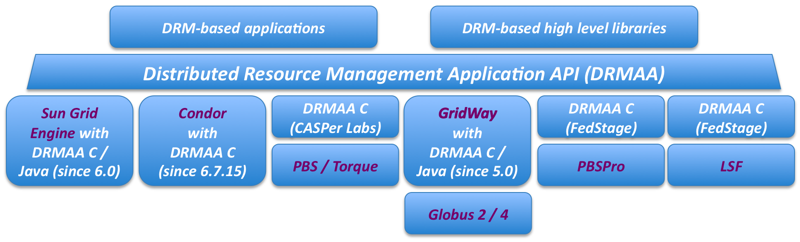
\includegraphics[width=9cm]{img/drmaastack.png}
	\end{center}


}
\frame{
\frametitle{Interfaces}

\begin{block}{}
  \begin{itemize}
    \item Interface commande en ligne (CLI)
    \item Application exemple DRMAA (v1, v2)
    \item Grille : Globus GT2, GT4/ OGSA-BESS, G-Lite - BLAHp, SAGA
    \item Interface web REST
    \item avec des jolies variantes
  \end{itemize}
 \end{block}

	\begin{center}
			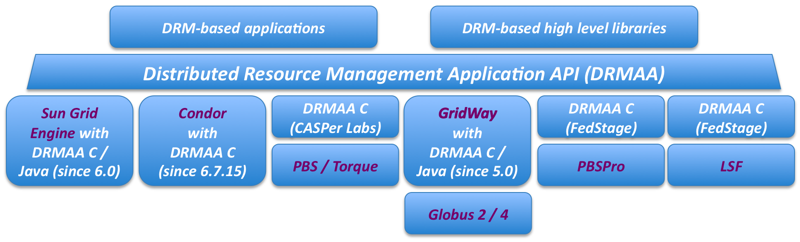
\includegraphics[width=9cm]{img/drmaastack.png}
	\end{center}


}



\begin{frame}
  \frametitle{Interface web : REST} 
  \begin{block}{}
    \begin{itemize}
      \item REST = protocole HTTP PUT/GET/POST/DELETE sur des ressources 
      \item \url{http://fr.wikipedia.org/wiki/Representational_State_Transfer}
      \item interface simplifiée
      \item  présent dans OAR (apparitions dans d'autre gestionnaire LAVA, SGE ???)  
    \end{itemize}
  \end{block}
%\begin{verbatim}
%# Get the list of resources
%wget -O - http://mydomain.org/oarapi/resources.yaml?structure=simple
%\end{verbatim}

wget -O -
\url{http://mydomain.org/oarapi/resources.json?structure=simple}
Donne la liste de toutes les ressources de la grappe au format json 

\end{frame}



\section{Energie}

\begin{frame}
  \frametitle{Energie}
\end{frame}


\begin{frame}
  \frametitle{The Green500 List}
    Machines du Top500 triées suivant les Mflops/Watt


    \begin{center}
      \includegraphics[height=7cm]{img/green500.png}
    \end{center} 

\end{frame}

\begin{frame}
  \frametitle{The Green500 List}
  \begin{itemize}
		\item Les architectures spécialisées occupent les 19 premières places.
    \item Machine {\em classique}: Blade Center Xeon QC 2.5 Ghz ({\bf 265.80 MFlops/Watt}).
    \item Le benchmark utilisé (Linpack) est bien connu et bien maîtrisé !
    \item Pas de données pour des benchmarks plus variés.
    \item Les informations sur la puissance consommée font leur apparition dans le Top500.  
   \end{itemize}
\end{frame}

\begin{frame}
  \frametitle{Quelques puissances consommées}
  \includegraphics[height=1cm]{img/banniere_greennet.jpg}
  Projet INRIA sur le suivi de la consommation et l'étude des logiciels pour sa maîtrise dans le HPC.
  \begin{center}
      \includegraphics[height=5cm]{img/green-net-002.jpg}
      \end{center} 

\end{frame}

\begin{frame}
  \frametitle{Quelques consommations}
 
  \begin{center}
    \includegraphics[height=5cm]{img/green-net-003.jpg}
  \end{center} 

\end{frame}

\begin{frame}
  \frametitle{Autres consommations}
  2 machines bi-quad-core Xeon (BULL)
  \begin{center}
    \includegraphics[height=3cm]{img/genepi-power/genepi-month.png}
  \end{center} 
  \begin{center}
    \includegraphics[height=3cm]{img/genepi-power/genepi-year.png}
  \end{center} 
\end{frame}

\begin{frame}
  \frametitle{SGI Molecule: Concept Computer}
  Présentée à SC'08.
  \begin{center}
    \includegraphics[height=3cm]{img/SGI_Molecule.jpg}
  \end{center} 

	\begin{itemize}
		\item Intel Atom N330
    \item Rack 3U, 90 noeuds / rack , 5-10 Watts / noeud 
  \end{itemize}

  \begin{itemize}
		\item Autre société, Sicortex: 5,832 cpu (64bits MIPS 1,4 Gflops), 20KWatt
    \item ARM processeur dual-core Cortex A-9  / 2Ghz / 0.5 Watt (FPU ???)
  \end{itemize}

\end{frame}

\begin{frame}
  \frametitle{Centre de calcul, mésocentre, grappes labo, grappes pour l'expérimentation}
  \begin{itemize}
		\item Des rôles très variés
    \begin{itemize}
      \item Régles d'usages, durée des jobs, type de jobs...    
    \end{itemize}

    \item Des taux d'utilisation différents / consommations énergiques
    \begin{itemize}
      \item $90\% - 100\%$ pour les centres de calcul (?).
      \item Plus variable pour les méso-centres.
      \item Très irrégulier pour les grappes de labo et les plate-formes pour l'expérimentation comme Grid'5000 ($25\% - 50\%$).
      \item Utilisation des ressources inutilisées pour les applications paramétriques (généralement en mode {\bf BestEffort}), mais il reste de large périodes d'inactivité. 
    \end{itemize}
  \end{itemize}
\end{frame}



\begin{frame}
  \frametitle{Centre de calcul et Energie}
  \begin{itemize}
		\item Maximiser le rendement énergetique (pas forcément la priorité). 
    \item Le matériel est-il bien adapté, efficace... ?
    \item Quel est le rendement des applications (accélération, gaspillage) ? (rarement connu, ou peu surveillé) 
    \item La gestion globale des ressources permet-elle une bonne maîtrise de la consommation d'énergie ? (les détails de la consommation ne sont que rarement connus)
  \end{itemize}
\end{frame}

\frame{
  \begin{center}
    Quelques études de cas liées à la consommation d'énergie.
  \end{center}
}

\begin{frame}
  \frametitle{Seuil de température}
  \begin{itemize}
		\item Cas d'une climatisation limite.
    \item Lors d'un pic de température nécessité d'arrêter ou de mettre en veille des noeuds.
    \item La sonde de température alerte le gestionnaire de ressource (puis IPMI ou script de mise en veille).
    \item Arrêt de noeud libre, noeud avec job besteffort, checkpoint avant retrait du job et arrêt du noeud ou arrêt du noeud et perte du job.
    \item {\em Simple à mettre en place dans un gestionnaire de ressource.}
  \end{itemize}
\end{frame}

\begin{frame}
  \frametitle{Cluster Virtuel - ComputeMode}
  \includegraphics[height=2cm]{img/Logo_ComputeMode.png}

  \begin{itemize}
		\item Création d'un cluster virtuel avec les ressources inutilisées
    \item Exemple salle de TP la nuit (UFRIMA - Université Joseph Fourier)
    \begin{itemize}
      \item PXE
      \item Wake-On-Lan
      \item Diskless systems
      \item OAR comme gestionnaire de ressources, {\bf réveil à la demande, zone indisponible}
    \end{itemize}
    \item {\bf Usage: cluster d'appoint intégré dans la grille du Méso-centre CIMENT }
    \item {\bf Heure creuse, pas de climatisation, disques inutilisés ! :) }
  \end{itemize}

\end{frame}

\begin{frame}
  \frametitle{DSLlab}
  \begin{itemize}
		\item Plateforme pour l'expérimentation sur Internet/ réseau ADSL.
    \item Machine fanless chez les particuliers.
    \item Les machines sont en veille lorsqu'elles sont inutilisées (pas de  Wake-On-Lan
possible)
     \item Fonction d'{\bf heure de réveil} par les carte-mères (géré via par le gestionnaire de ressource) 
  \end{itemize}
\end{frame}


\section{Les propositions actuelles}

\begin{frame}
  \frametitle{Arrêt / Mise Veille / Réveil}
  \begin{itemize}
		\item Arrêt / Mise Veille des noeuds lorsqu'ils sont inutilisés
    \item Réveil lors de l'arrivée de nouveau job
    \item Limiter les cycle d'arrêts/réveil (réactivité) $\rightarrow$ prédire la charge.
    \item {\bf Note:} Arrêt/allumage de machines fatiguent peu le matériel (15000 cycles arrêt brutal/allumage pas de souci particulier).
    \item {\em Assez simple à mettre en place dans un gestionnaire de ressource.}
 
  \end{itemize}
\end{frame}

\begin{frame}
  \frametitle{Tarifications heures pleines/creuses - Tâche Priotaire }
  \begin{itemize}
		\item Les tâches prioritaires passent en journée en heures pleines.
    \item Toutes les tâches peuvent passer la nuit en heures creuses.
    \item Variantes: des noeuds sont éteints en journée ou bloqués à vitesse réduite (consommation limitée, {\bf attention, par forcément le plus efficace en énergie consommée, durée/efficacité})
    \item {\em Assez simple à mettre en place dans un gestionnaire de ressource.}
 

   \end{itemize}
\end{frame}


\begin{frame}
  \frametitle{Slurm}
  Approche simple
  \begin{itemize}
		\item {\bf SuspendTime:} nombre de seconde à partir duquel un noeud peut être mise en veille / éteint 
    \item {\bf SuspendRate, ResumeRate:} nombre de noeud par minute pouvant changer d'état (important pour les grosses installation) 
    \item {\bf SuspendProgram, ResumeProgram:} programme à exécuter pour contrôler les noeuds
    \item {\bf SuspendExcNodes, SuspendExcParts:} noeuds et/ou partition à exclure du contrôle
  \end{itemize}
\end{frame}

\begin{frame}
  \frametitle{LSF, Moab (Cluster Resources) }
  Attention pas testé, document très commercial pour Moab, factuel pour LSF
  \begin{itemize}
		\item Suivi de consommation, température
    \item Usage de consommation par utilisateur, projet, job (?)
    \item Gestion/contrôle d'énergie
    \begin{itemize}
      \item arrêt/mise en veille de noeud
      \item priorité heures creuses/ heures pleines
    \end{itemize}
  \end{itemize}
\end{frame}

\begin{frame}
  \frametitle{OAR et gestion de l'énergie}
  \begin{itemize}
    \item Priorité heures creuses/pleines par paramétrage
		\item Développées lors du {\em Google Summer Of Code 2008} (Gsoc'08)
    \begin{itemize}
       \item Module de prédiction de charge.
       \item Un nouveau type de job paramétrique:  {\bf powersaving} + options (cpufreq, arrêt sélectif de périphérique disque, video ..., politique spécifique)
       \item Ex Job BestEffort $\rightarrow$ fréquence CPU la plus faible.
    \end{itemize}
  \end{itemize}
\end{frame}

\frame{
	\begin{center}
    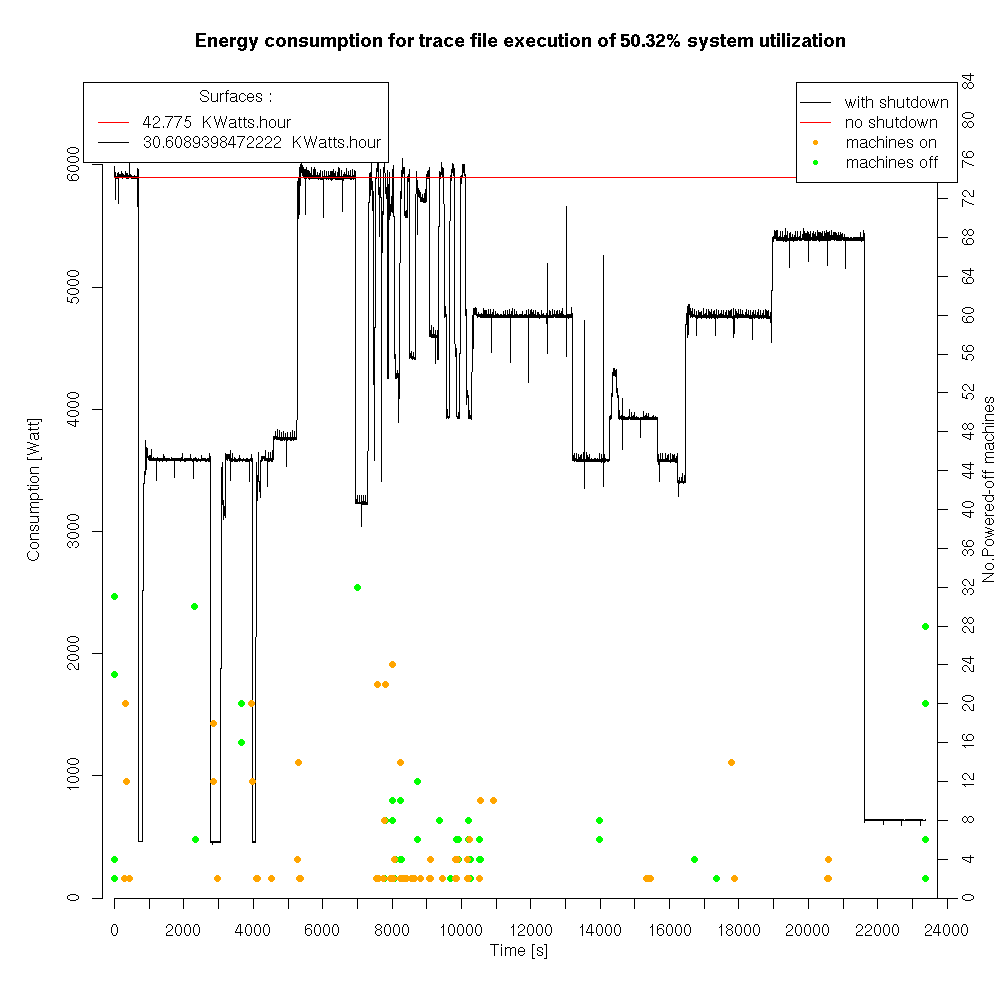
\includegraphics[width=9cm]{img/energy50.png}
  \end{center}

}

\frame{
  \begin{center}
    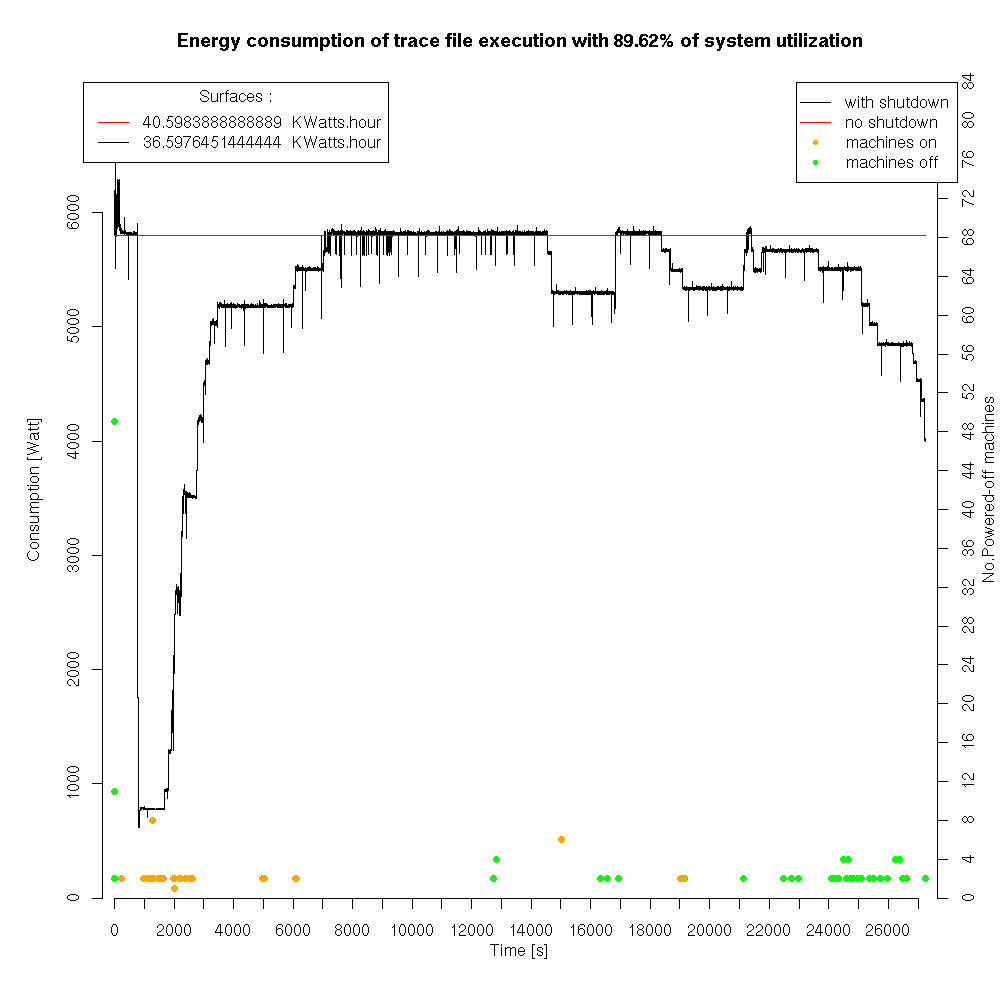
\includegraphics[width=9cm]{img/energy90.png}
  \end{center}
}








\section{Du coté des applications et du système}

\begin{frame}
  \frametitle{Du coté des applications et du système}
  Des travaux de recherches;
  \begin{itemize}
    \item Contention mémoire, concurrence et consommation.
		\item Application MPI et contention (10\% conso en moins, 1\% de temps en plus).
    \item DVFS et opérations I/O.
    \item Consommation et machines virtuelles (vision intégré).
    \item Répartition de charge au niveau des grilles.
   \end{itemize}
\end{frame}

\begin{frame}
  \frametitle{En pratique}
  \begin{itemize}
		\item La sélection du matériel, monitoring précis de la consommation.
    \item Bien connaître les applications (bon rendement énergétique).
    \item Discussion avec les utilisateurs (pour la maîtrise du gaspillage, qualité du code)
    \item Politique {\em de gestion d'énergie}: arrêt/mise en veille, priorité, heures pleines/ heures creuses, 
    \item Veille technologique...  
  \end{itemize}
\end{frame}



\section{Divers}

%TODO Equilibrage LoadBalancing


\frame{
\frametitle{Divers}
}

\begin{frame}
	\frametitle{Divers cas d'exploitation}
	\begin{itemize}
		\item Applications Multiparamétriques
				\begin{itemize}
					\item Utilisation des ressources non-utilisées
				\end{itemize}

		\item Déploiement/Virtualisation
				\begin{itemize}
				  \item Des ressources plus simples à exploiter pour les utilisateurs	
				\end{itemize}
		\item Ressources hétérogénes 
				\begin{itemize}
				  \item mémoire
					\item réseaux
					\item licence
				\end{itemize}
		\item Tolérance aux pannes
		\item Haute-disponibilité
		\item Multi-grappes
	\end{itemize}
\end{frame}


\begin{frame}
	\frametitle{Haute-disponibilité}
	Assurer la continuité de service est important pour les grandes infrastructure

	\begin{block}{Pannes d'un noeud de calcul:}
	\begin{itemize}
	  \item Arrêt en erreur de la tâche  (nettoyage des autres noeuds)
		\begin{itemize}
  		\item re-soumission automatique (si option positionnée)
			\item reprise depuis un point de reprise si disponible ({\em checkpointing})
		\end{itemize}
	\end{itemize}
  \end{block}

  \begin{block}{Pannes du seveur:}

	  \begin{enumerate}
  	  \item maintient d'un second serveur (synchronisation d'état), bascule auto
 		  \item élection d'un nouveau serveur parmi les noeuds de calcul (LSF)
	  \end{enumerate}
  \end{block}

{\bf Note:} Suppose la HA sur les autres services critiques comme l'authentification (ex Ldap), le système de fichier distribué (ex NFS) (exemple SGE), de nommage (ex DNS), BD (OAR)...

\end{frame}

\begin{frame}
	\frametitle{Multi-grappe}
	Le cas des multi-grappes est très courant:
		\begin{enumerate}
  		\item achat d'une nouvelle grappe et conservation de l'ancienne 
 			\item achat par tranche
		\end{enumerate}
	Deux approches distinctes:
		\begin{enumerate}
  		\item un gestionnaire par grappe
			\begin{itemize}
  			\item file de routage vers les autres gestionnaire de tâches/ressources
			\end{itemize}

 			\item un seul gestionnaire pour l'ensemble des grappes \footnote{C'est le cas pour Grid'5000, 3 à 5 grappes par site}
			\begin{itemize}
  			\item chaque grappe est vue comme une partition homogéne dans l'ensemble des ressources
				\item suppose ({\em pousse pour}) que les services soient commun à chaque grappe (ex: système de fichier, authentification,...)
				\item simplifie énormément l'administration
			\end{itemize}
			 
		\end{enumerate}

\end{frame}



\begin{frame}
	\frametitle{Cas des longues tâches}
		
		\begin{enumerate}
			\item Dédier des noeuds
			\item Suspendre en journée / relancer la nuit ou le week-end
			\item Checkpoint (point de reprise)
			\begin{itemize}
				\item applicatif (la solution la plus sûre)
				\item système (contraintes, limitations)
			\end{itemize}
		\end{enumerate}

\end{frame}

\section{GUI}

\frame{
\frametitle{GUI}
  
}

\frame{
\frametitle{SGE: Xml-qstat}
\includegraphics[width=\textwidth]{img/xml-qstat.jpg}

}

\frame{
\frametitle{OAR: Diagramme de Gantt}
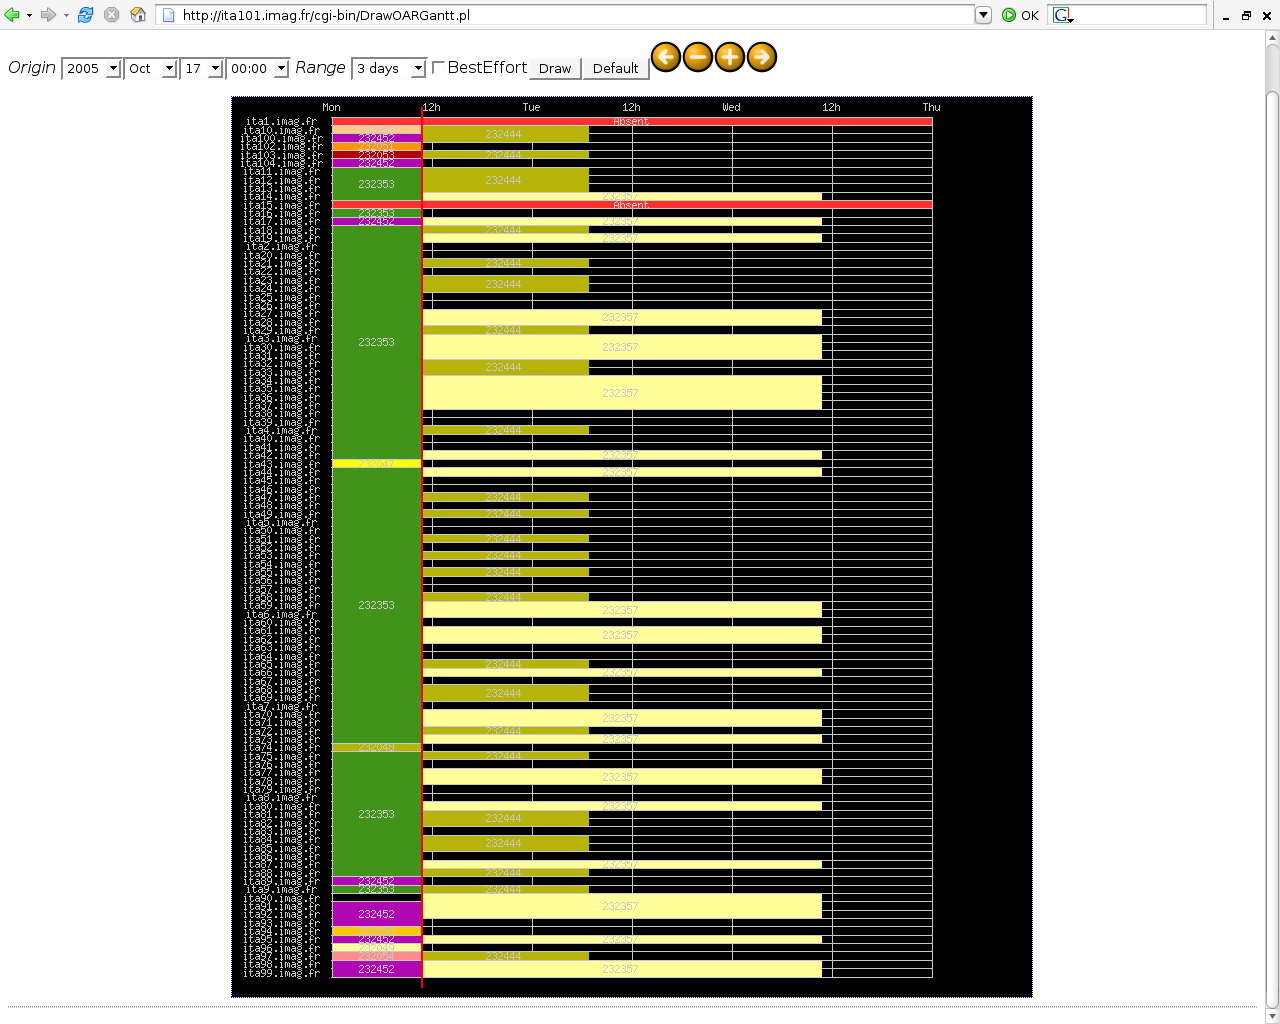
\includegraphics[width=\textwidth]{gantt_ita.png}

}

\frame{
\frametitle{ClusterVisionOS: une vision intégrée}
\includegraphics[width=\textwidth]{ClusterVisionOS_screenshot.png}
}


\frame{
  \frametitle{Eléments de comparaison \alert{(Forcément biasé !!!)}}

  \begin{itemize}
    \item {\bf Condor} référence académique (High-Throughput Computing) 
		\item {\bf Sun Grid Engine (SGE)} vieillissant / vraiment libre ? 
    \item {\bf MAUI/Torque} vieillissant / vraiment libre ? 
    \item {\bf Slurm} {\bf très grandes machines}
    \item {\bf OAR} {\bf Challenger } :)
    \item LSF (Platform) (pour le support)
    \item PBS Pro (pour le support)
  \end{itemize}

\begin{block}{C'est aussi une affaire de goût ?}
  \begin{itemize}
    \item Différence dans la philosophie: exemple OAR définit ressources exemple les cores, les licences, SGE dédinit des queue, des hosts auxquels sont rattachés des ressources 
  \end{itemize}
\end{block}


}



 
\section{Conclusion}
\begin{frame}
\frametitle{Conclusion}

Ce qu'il faut retenir:

\begin{itemize}
	\item Les grappes sont quasi-ominiprésentes dans le domaine des sciences appliquées.
	\item Leur taille augmente
	\item Les gestionnaires de tâches et de ressources sont nécessaires
	\item {\bf Fixer une politique de partage et d'accès}
	\item {\bf Dialoguer/Former/Informer les utilisateurs (réunion d'information,documentation, chartre, tutoriaux...)}
	\item Des gestionnaires de ressources pour tout les goûts (logiciels libres et propriétaires)
	\item Le réglage fin reste {\bf complexe} (les infrastructures sont complexes, et les demandes aussi). Beacoup de compromis.
 \end{itemize}
\end{frame}

\begin{frame}
	\begin{center}
		{\huge Des questions ?}
	\end{center}
\end{frame}

\begin{frame}
\frametitle{Liens}
\begin{thebibliography}{Resource Management System}

	\bibitem{Condor}
	Condor 
	\newblock {\em http://www.cs.wisc.edu/condor/}

  \bibitem{SGE}
	Sun Grid Engine (SGE) 
	\newblock {\em http://gridengine.sunsource.net}

	\bibitem{TORQUE}
	TORQUE/MAUI
	\newblock {\em http://www.clusterresources.com/}

  \bibitem{SLURM}
	SLURM
	\newblock {\em www.llnl.gov/linux/slurm/}

	\bibitem{LSF}
	LSF
	\newblock {\em http://www.platform.com}

	\bibitem{OAR}
	OAR 
	\newblock {\em http://oar.imag.fr}



\end{thebibliography}
\end{frame}

\end{document}

